\documentclass[dvipdfmx]{article}
\usepackage[dvipdfmx]{graphicx}
\usepackage{amsmath, amssymb}
\usepackage{mathtools}
\usepackage{here}
\begin{document}
\title{Weekly Report}
\author{Riku Gondow}
\maketitle
\section{Progress}
\begin{itemize}
    \item Visualize feature mapping
    \item (Set up the assigned server)
\end{itemize}

\section{Feature Mapping}
Below are images of the feature mapping at the final stage of training. (Animations showing the mapping changes is attached to the e-mail.)
The extracted features were dimensionally reduced using t-SNE. The plots with the same color are the same class, and the plots with different colors are different classes. The number of classes is 15.


\begin{figure}[H]
\begin{center}
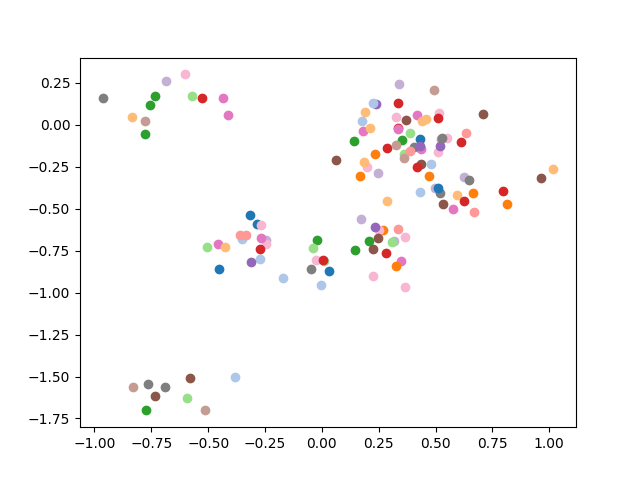
\includegraphics[width=0.8\linewidth]{./img/Cross_300_01_Fmap.png}
\end{center}
\caption{Feature mapping for CrossEntropy Loss(Conventional method)}
\end{figure}

\begin{figure}[H]
\begin{center}
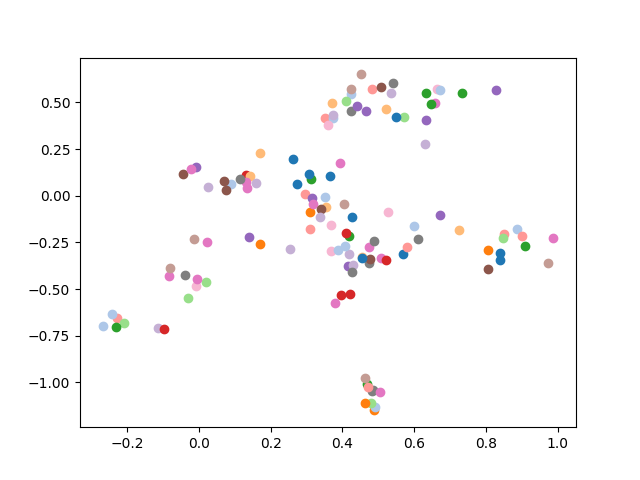
\includegraphics[width=0.8\linewidth]{./img/Center_300_01_Fmap.png}
\end{center}
\caption{Feature mapping for Center Loss + Softmax Loss(Most accurate method)}
\end{figure}

\begin{figure}[H]
\begin{center}
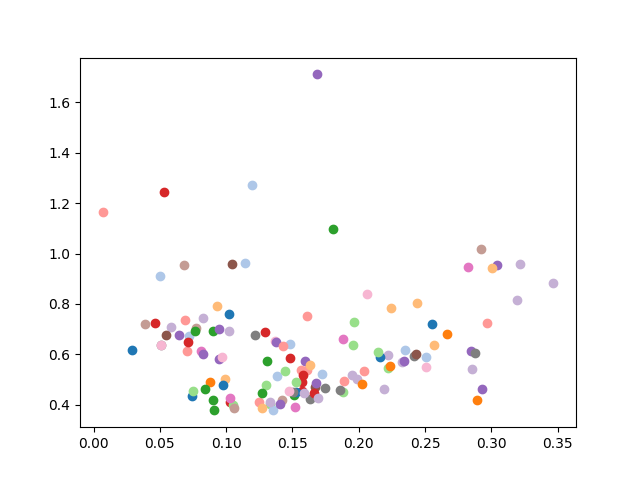
\includegraphics[width=0.8\linewidth]{./img/Cos_300_01_Fmap.png}
\end{center}
\caption{Feature mapping for Cosine Loss + Center Loss + Softmax Loss (=Triple Joint Loss)}
\end{figure}

Although there is some variation in CenterLoss and CrossEntropyLoss, we could not observe clusters in each class. There are several possible reasons for this.
\begin{enumerate}
    \item Loss of information due to compression of the 15-dimensional features to two dimensions.
    \item The code is incorrect.
    \item The model includes a batch normalization layer, which makes it difficult to observe the separation of features.
\end{enumerate}

\section{Next Plan}
\begin{itemize}
    \item Verify the visualization code
    \item Check the noisy dataset
    \item Consider methods for noisy dataset
    \begin{itemize}
        \item Survey preprocessing methods
        \item Discuss preprocessing methods with Xing-San and Kai-San
        \item Implement Openmax and Proportional Similarity-based Openmax
    \end{itemize}
\end{itemize}
\end{document}